\section{Coupled-GRPO}
\label{sec:grpo}
Reinforcement learning (RL) and GRPO~\citep{shao2024deepseekmath} have proven critical for enhancing AR models~\citep{bercovich2025llama,shao2025spurious}, but their application to dLLMs is less explored. 
As discussed in \S\ref{sec:pre-grpo}, formulating the mask diffusion process as a Markov Decision Process allows for a policy optimization approach akin to PPO~\citep{schulman2017proximal}. 
To facilitate integration with GRPO~\citep{shao2024deepseekmath}, the approximation of token probabilities within diffusion models is necessary. 
Current masked diffusion models rely on Monte Carlo sampling~\citep{li2025llada, shi2024simplified} for log-probability estimation. 
Specifically, the negative log-likelihood (NLL) is bounded by the ELBO, \textit{i.e.}, $\mathcal{P}_i = \mathbb E_{t\sim1,...T;\bm{x}_t\sim q(\bm{x}_t|\bm{x}_0)} [\mathcal{L}_{t}(\bm{x}_t)]$, where $\mathcal{L}_{t}$ is the cross-entropy loss introduced in Eq.~(\ref{eq:dm-loss}). 
However, Monte Carlo sampling introduces significant overhead during the training of GRPO, as highlighted by d1~\citep{zhao2025d1}. 
\paragraph{Baseline methods}
To overcome this, d1 chooses to mask all completion tokens and perform a single forward pass to compute each token's probability, which is equivalent to sampling once at diffusion step $t=T$; we call this sequence of log-probabilities $\mathcal P_i$, with each element being $\log\pi_\theta(o_i^k|c,o_i^k=\bm{m})$. 
Thus, GRPO's update in Eq.~(\ref{eq:grpo-loss}) uses the ratio $\rho_i^k =\frac{\pi_\theta(o_i^k| c,o_i^k=\bm{m})}{\pi_{\theta_\text{old}}(o_i^k| c,o_i^k=\bm{m})}$.
d1 also randomly masks $p=15\%$ of the condition tokens to increase sampling diversity, which, in practice, makes the completion-token probability estimates unreliable. 
In our code experiments, masking condition tokens does not yield a stable reward improvement (Figure~\ref{fig:grpo-compare}), probably because code tasks demand higher token-level generation accuracy than math tasks. 
As a result, we revert to the \emph{completion full mask} version ($p=0\%$) and use $\mathcal P_{t=T}$ as our baseline. 
Even so, this baseline is biased: as shown in our \emph{entropy sink} analysis (\S\ref{sec:analysis}), high-entropy tokens tend to lie on the left side, so RL training still ends up updating early tokens more aggressively.
\paragraph{Coupled-GRPO}
In the $\mathcal{L}_{t}$ computation, only the loss for positions involving masked tokens is counted, which introduces inefficiency and variance when sampling times are limited. 
To improve probability estimation while still covering every token, we introduce a coupled-sampling scheme (Figure~\ref{fig:pipeline}). 
Concretely, we pick $\lambda$ timestep pairs $(t, \hat{t})$ with $t+\hat{t}=T$, then sample two complementary completion masks: each mask hides part of the tokens, and together they cover all completion tokens. 
In other words, every token is unmasked in exactly one of the two forward passes. 
This design guarantees that (1) each token's log-probability is computed at least once (giving each token a non-zero learning signal) and (2) these log-probability estimations are more accurate because every token is evaluated under a realistic partial-masking context rather than always being masked, and we have $2\lambda$ additional samples compared to the baseline. Combining Eqs.~(\ref{eq:dm-loss}), (\ref{eq:ddpo-loss}), and (\ref{eq:grpo-loss}), we have:
{
\small
\begin{align}
&\mathcal J_{\text{GRPO}}(\theta)= 
\mathbb E\Bigl[\sum_{i=1}^G\sum_{k=1}^{|o_i|}
  \min\Bigl(\frac{\pi_\theta(o_i^k| c,o_{i,t<T}^k)}{\pi_{\theta_\text{old}}(o_i^k| c,o_{i,t<T}^k)} A_i,\mathrm{clip}\bigl(\frac{\pi_\theta(o_i^k| c,o_{i,t<T}^k)}{\pi_{\theta_\text{old}}(o_i^k|c,o_{i,t<T}^k)},1-\varepsilon,1+\varepsilon\bigr)A_i\Bigr)-\beta\KL\Bigr],\notag\\
  &\text{with }\log\pi_\theta(o_{i}^k| c,o_{i,t<T}^k) = \frac{1}{\lambda+1}\bigg[\sum_{t+\hat{t}=T}^{\lambda}[\mathcal{L}_{t}(\bm{x}_t) + \mathcal{L}_{\hat{t}}(\bm{x}_{\hat{t}})] + \mathcal{L}_{T}(\bm{x}_T)\bigg]_i^k, \;\delta_{\bm{x}_t,\bm{m}}+\delta_{\bm{x}_{\hat{t}},\bm{m}}=\bm{1}.
  \label{eq:grpo-loss-cp}
\end{align}
}

In practice, we choose $\lambda=1$. For a fair comparison, we introduce a de-coupled baseline with the same number of samples but without the complementary constraint.
For advantage score computation, we also consider leave-one-out (LOO) strategies~\citep{ahmadian2024back,kool2019buy} to determine the baseline score: $A_i=r(o_i)-\frac1{G-1}\sum_{j\neq i}^{G} r(o_j)$, which creates an unbiased estimate. 
We show that our coupled-sampling scheme can be viewed as an application of the Antithetic Variates~\citep{hammersley1956general} variance reduction technique in Appx.~\ref{appx:coupled-grpo}, where we also list detailed designs for verified rewards, including a code format reward and the execution pass rate over test cases as a correctness reward.

\begin{figure}[ht]
  \centering
  \begin{subfigure}[c]{0.32\textwidth}
    \centering
    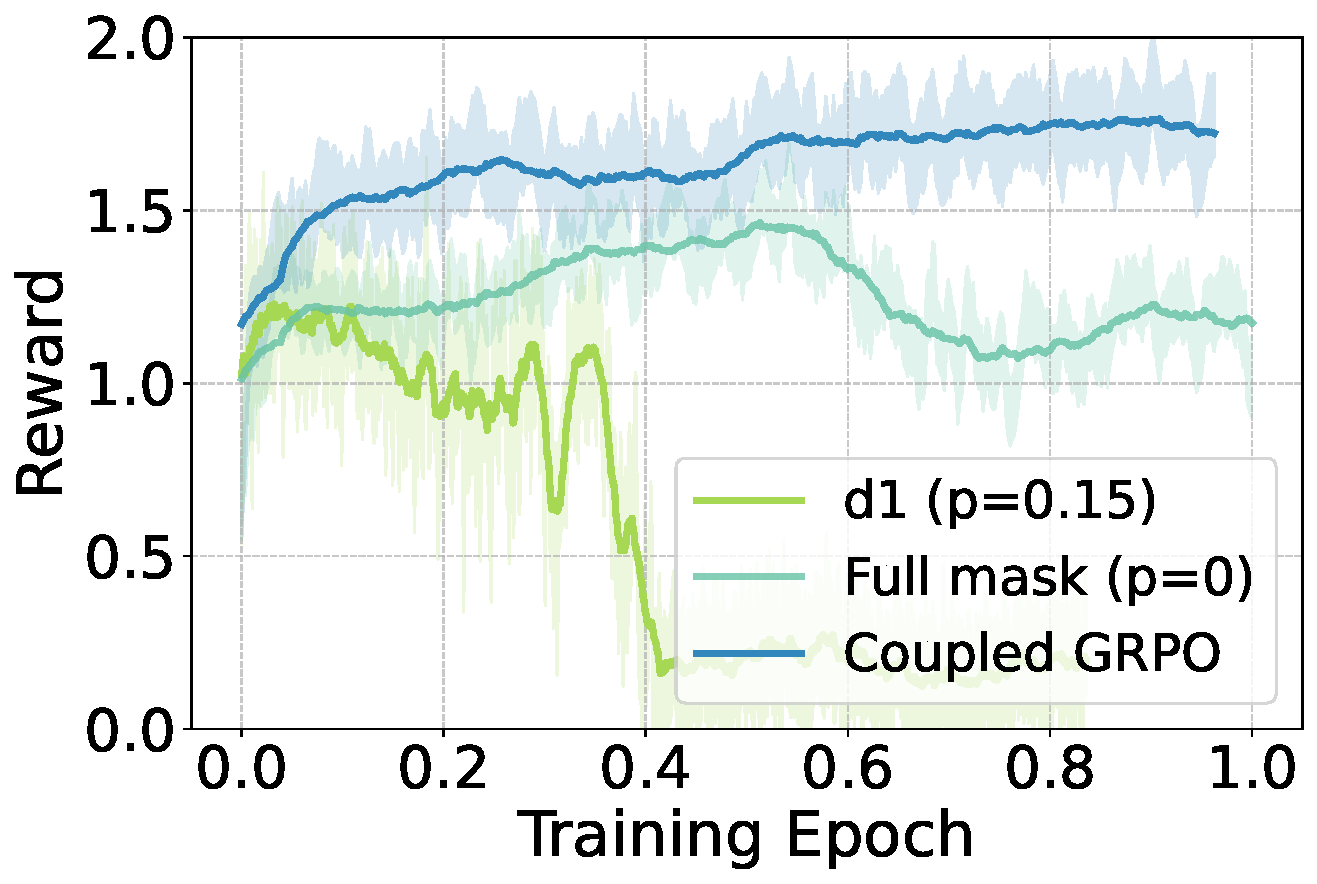
\includegraphics[width=\linewidth]{fig/reward_curves_d1-2.pdf}
  \end{subfigure}
  \hfill
  \begin{subfigure}[c]{0.32\textwidth}
    \centering
    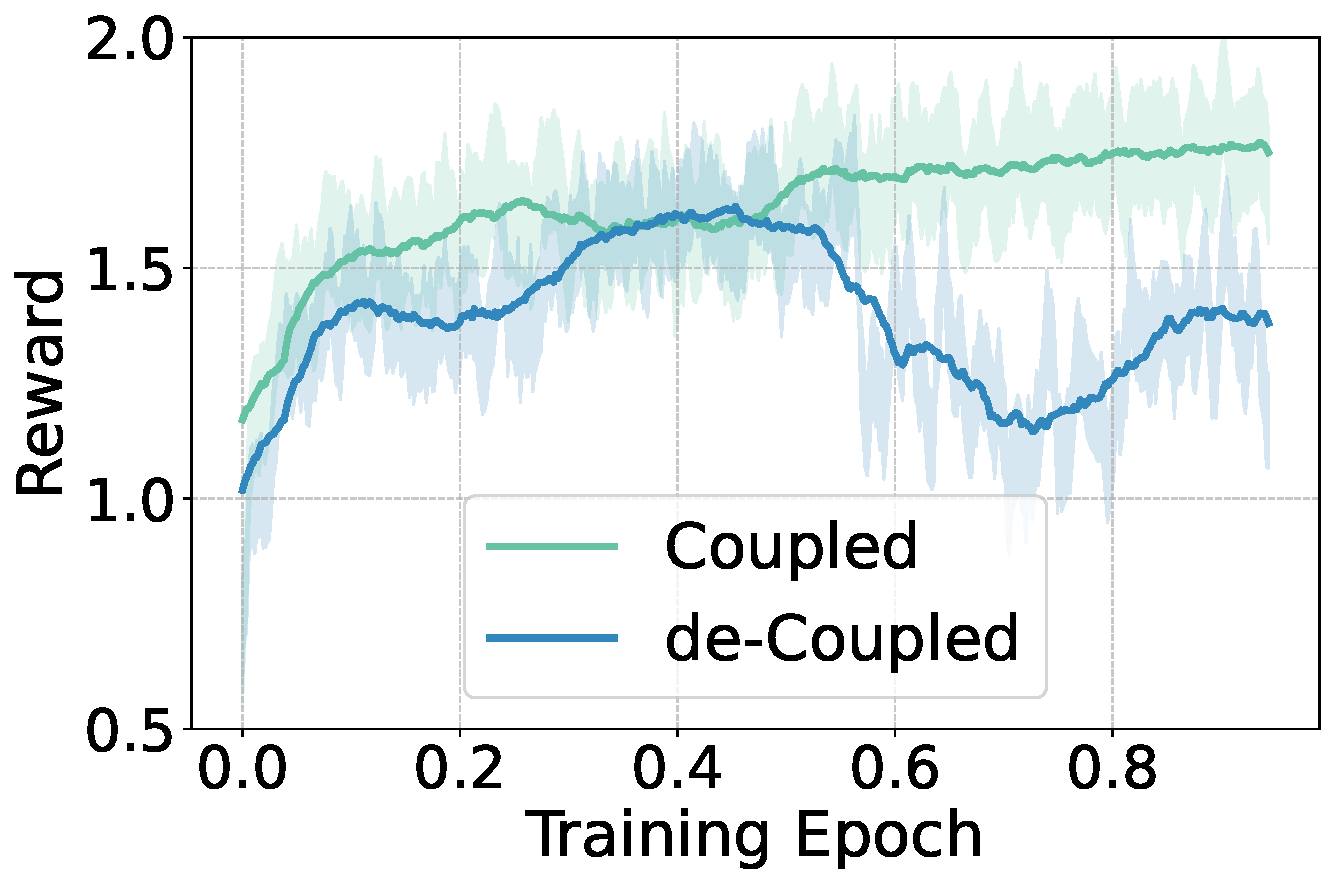
\includegraphics[width=\linewidth]{fig/reward_curves_cp2.pdf}
  \end{subfigure}
  \hfill
  \begin{subfigure}[c]{0.32\textwidth}
    \centering
    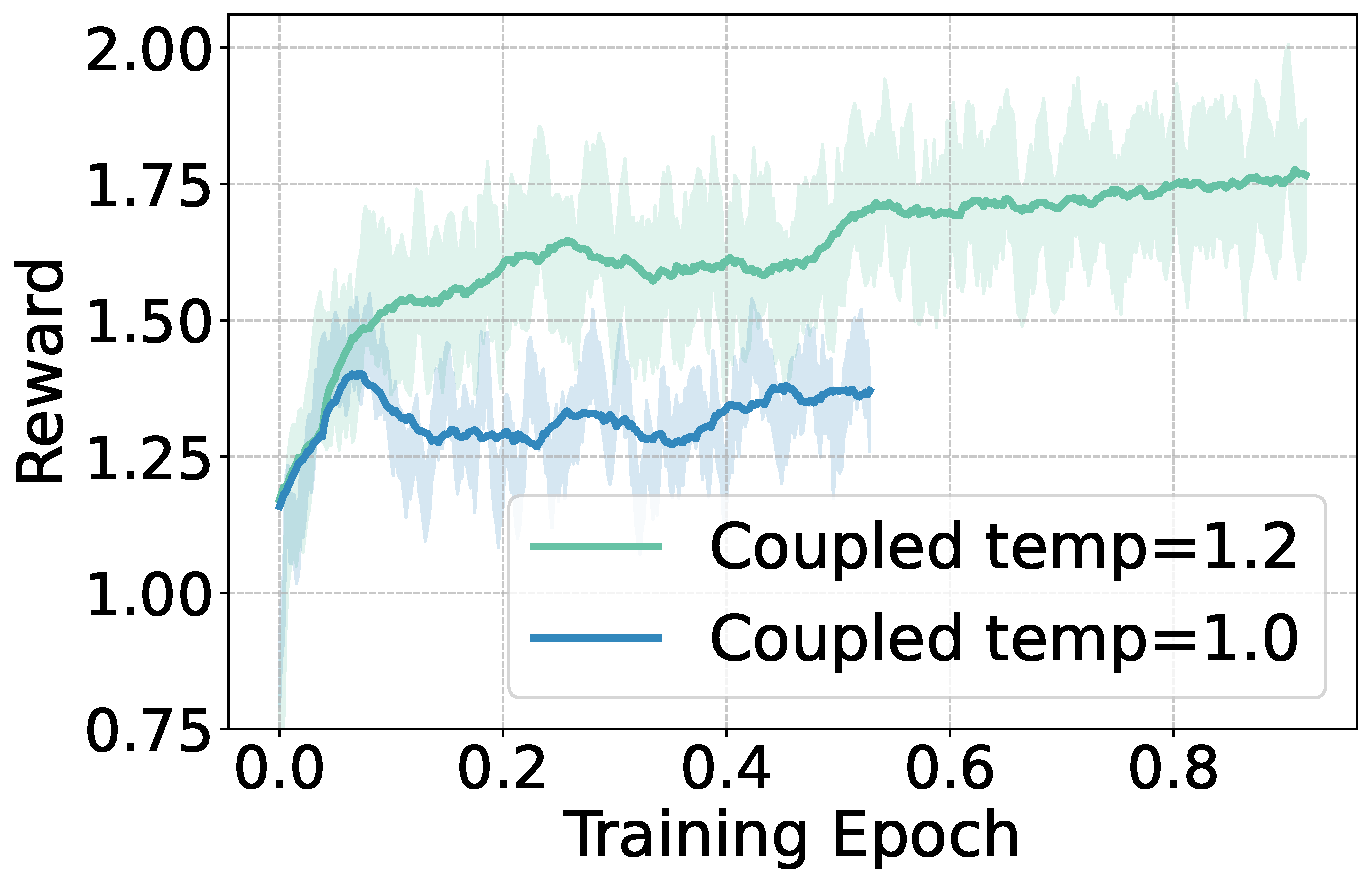
\includegraphics[width=\linewidth]{fig/reward_curves_temp.pdf}
  \end{subfigure}
  \caption{Reward curves during GRPO training. \textbf{Left}: Comparison between coupled GRPO and d1 baselines. \textbf{Middle}: Decoupled GRPO uses the same number of samplings but with randomly sampled mask noise. \textbf{Right}: Coupled-GRPO is sensitive to the rollout temperature.}
  \label{fig:grpo-compare}
\end{figure}
\begin{table}[ht]
\centering
\small
\setlength{\tabcolsep}{3.5pt}
\begin{tabular}{lllllllllc}
\toprule
 & \multicolumn{2}{c}{HumanEval} & \multicolumn{2}{c}{MBPP} & \multicolumn{2}{c}{BigCodeBench (C)} & \multicolumn{2}{c}{BigCodeBench (I)} \\
Model & -- & Plus & -- & Plus & Full & Hard & Full & Hard \\
\midrule
Qwen2.5-Coder+SFT          & 82.9 & 75.6 & 80.1 & 66.1 & 46.9 & 16.2 & 39.5 & 14.9 \\
+ GRPO                     & 80.5{\tiny\textcolor{red}{–2.4}}
                           & 75.0{\tiny\textcolor{red}{–0.6}}
                           & 84.4{\tiny\textcolor{ForestGreen}{+4.3}}
                           & 72.8{\tiny\textcolor{ForestGreen}{+6.7}}
                           & 49.7{\tiny\textcolor{ForestGreen}{+2.8}}
                           & 16.2{\tiny \textcolor{ForestGreen}{0.0}}
                           & 40.0{\tiny\textcolor{ForestGreen}{+0.5}}
                           & 10.2{\tiny\textcolor{red}{–4.7}} \\
\midrule
DiffuCoder-Instruct        & 72.0 & 65.2 & 75.1 & 61.9 & 35.7 & 12.2 & 34.0 & 8.8  \\
+ coupled GRPO             & 73.2{\tiny\textcolor{ForestGreen}{+1.2}}
                           & 68.3{\tiny\textcolor{ForestGreen}{+3.1}}
                           & 78.6{\tiny\textcolor{ForestGreen}{+3.5}}
                           & 67.5{\tiny\textcolor{ForestGreen}{+5.6}}
                           & 40.4{\tiny\textcolor{ForestGreen}{+4.7}}
                           & 10.8{\tiny\textcolor{red}{–1.4}}
                           & 37.5{\tiny\textcolor{ForestGreen}{+3.5}}
                           & 10.8{\tiny\textcolor{ForestGreen}{+2.0}} \\
+ coupled GRPO (LOO)             & 70.7{\tiny\textcolor{red}{–1.3}}
                           & 62.2{\tiny\textcolor{red}{–3.0}}
                           & 79.6{\tiny\textcolor{ForestGreen}{+4.5}}
                           & 68.5{\tiny\textcolor{ForestGreen}{+6.6}}
                           & 41.2{\tiny\textcolor{ForestGreen}{+5.5}}
                           & 13.5{\tiny\textcolor{ForestGreen}{+1.3}}
                           & 37.6{\tiny\textcolor{ForestGreen}{+3.6}}
                           & 12.8{\tiny\textcolor{ForestGreen}{+4.0}} \\ 
\cdashline{1-9}[0.8pt/2pt]
\addlinespace
\quad w.\ full mask completion
                           & 66.5{\tiny\textcolor{red}{–5.5}}
                           & 59.1{\tiny\textcolor{red}{–6.1}}
                           & 77.0{\tiny\textcolor{ForestGreen}{+1.9}}
                           & 65.1{\tiny\textcolor{ForestGreen}{+3.2}}
                           & 38.0{\tiny\textcolor{ForestGreen}{+2.3}}
                           &  8.8{\tiny\textcolor{red}{–3.4}}
                           & 35.6{\tiny\textcolor{ForestGreen}{+1.6}}
                           & 13.5{\tiny\textcolor{ForestGreen}{+4.7}} \\
\quad w.\ decoupled sampling
                           & 68.9{\tiny\textcolor{red}{–3.1}}
                           & 62.8{\tiny\textcolor{red}{–2.4}}
                           & 78.3{\tiny\textcolor{ForestGreen}{+3.2}}
                           & 66.4{\tiny\textcolor{ForestGreen}{+4.5}}
                           & 40.4{\tiny\textcolor{ForestGreen}{+4.7}}
                           & 10.8{\tiny\textcolor{red}{–1.4}}
                           & 36.5{\tiny\textcolor{ForestGreen}{+2.5}}
                           & 10.8{\tiny\textcolor{ForestGreen}{+2.0}} \\
\bottomrule
\end{tabular}
\caption{Evaluation results for GRPO post-training across multiple benchmarks and models. We report the best results from the sampling temperature set $\{0.2,0.3,0.4\}$.}
\label{tab:grpo-results}
\end{table}

\paragraph{Experiment Results} Table~\ref{tab:grpo-results}, together with Figure~\ref{fig:grpo-compare}, demonstrates the effectiveness of coupled-GRPO training. 
In contrast, the baseline variants: d1, full-mask completion, and decoupled sampling, exhibit unstable reward learning. 
The rollout sampling temperature is also critical: as shown in Figure~\ref{fig:passk}, DiffuCoder-Instruct attains a higher pass@10 at temperature $1.2$ than at $1.0$, mirroring the trend observed during coupled-GRPO training. 
Notably, RL fine-tuning shifts the optimal sampling temperature from $0.2$ to a larger value, such as $0.3$ or $0.4$, during evaluation, indicating that training sharpens the per-token distribution. 
This finding aligns with recent results for AR LLMs~\citep{cui2025entropy,liu2025prorl,agarwal2025unreasonable}, suggesting that the approaches proposed in these works may also be generalizable to dLLMs. 
Finally, at the new optimal temperature, global decoding AR-ness decreases, as shown in Figure~\ref{fig:causal-stages} (right). A more interesting finding is that, as shown in Figure~\ref{fig:teaser}(c), when we use $0.5\times$ fewer decoding steps (equivalent to a $2\times$ generation speedup), training with coupled-GRPO results in a smaller performance drop compared to the model before training, suggesting that AR-ness is reduced and parallelism is increased~\citep{fastdllm2025}. Detailed discussions are provided in Appx.~\ref{sec:appx:decodet} and Appx.~\ref{sec:appx:discuss}.



